\section{Impedance analysis} \label{sec:ImpedanceAnalysis}
In order to measure, and analyze, an impedance it is important to have a clear definition of what impedance actually is. This sections will describe what an impedance is and how it can be used to analyze a device under test (DUT).

The impedance of a DUT, or circuit, is the devices ability to restrict the flow of alternating current and is the relationship between the current flowing through the DUT and the voltage across it. This can be visualized with a \textit{phasor} diagram. Phasors are vectors in the complex plane that represent sinewaves with a fixed amplitude and frequency. They are used to visualize phase shifts between different signals. For this analysis there will be voltage and current phasors as these can be used to find impedance phasors. Consider the case where the DUT is, mostly, capacitive in nature. In this case the current vector, $\bar i$, will lead the voltage vector $\bar v$ as shown on figure \ref{fig:4_1_CapPhasor}. \textit{lead} just means that the current has a positive phase shift relative to the voltage, if the opposite were true it would be \textit{lagging}.

\begin{figure}[H]
    \centering
    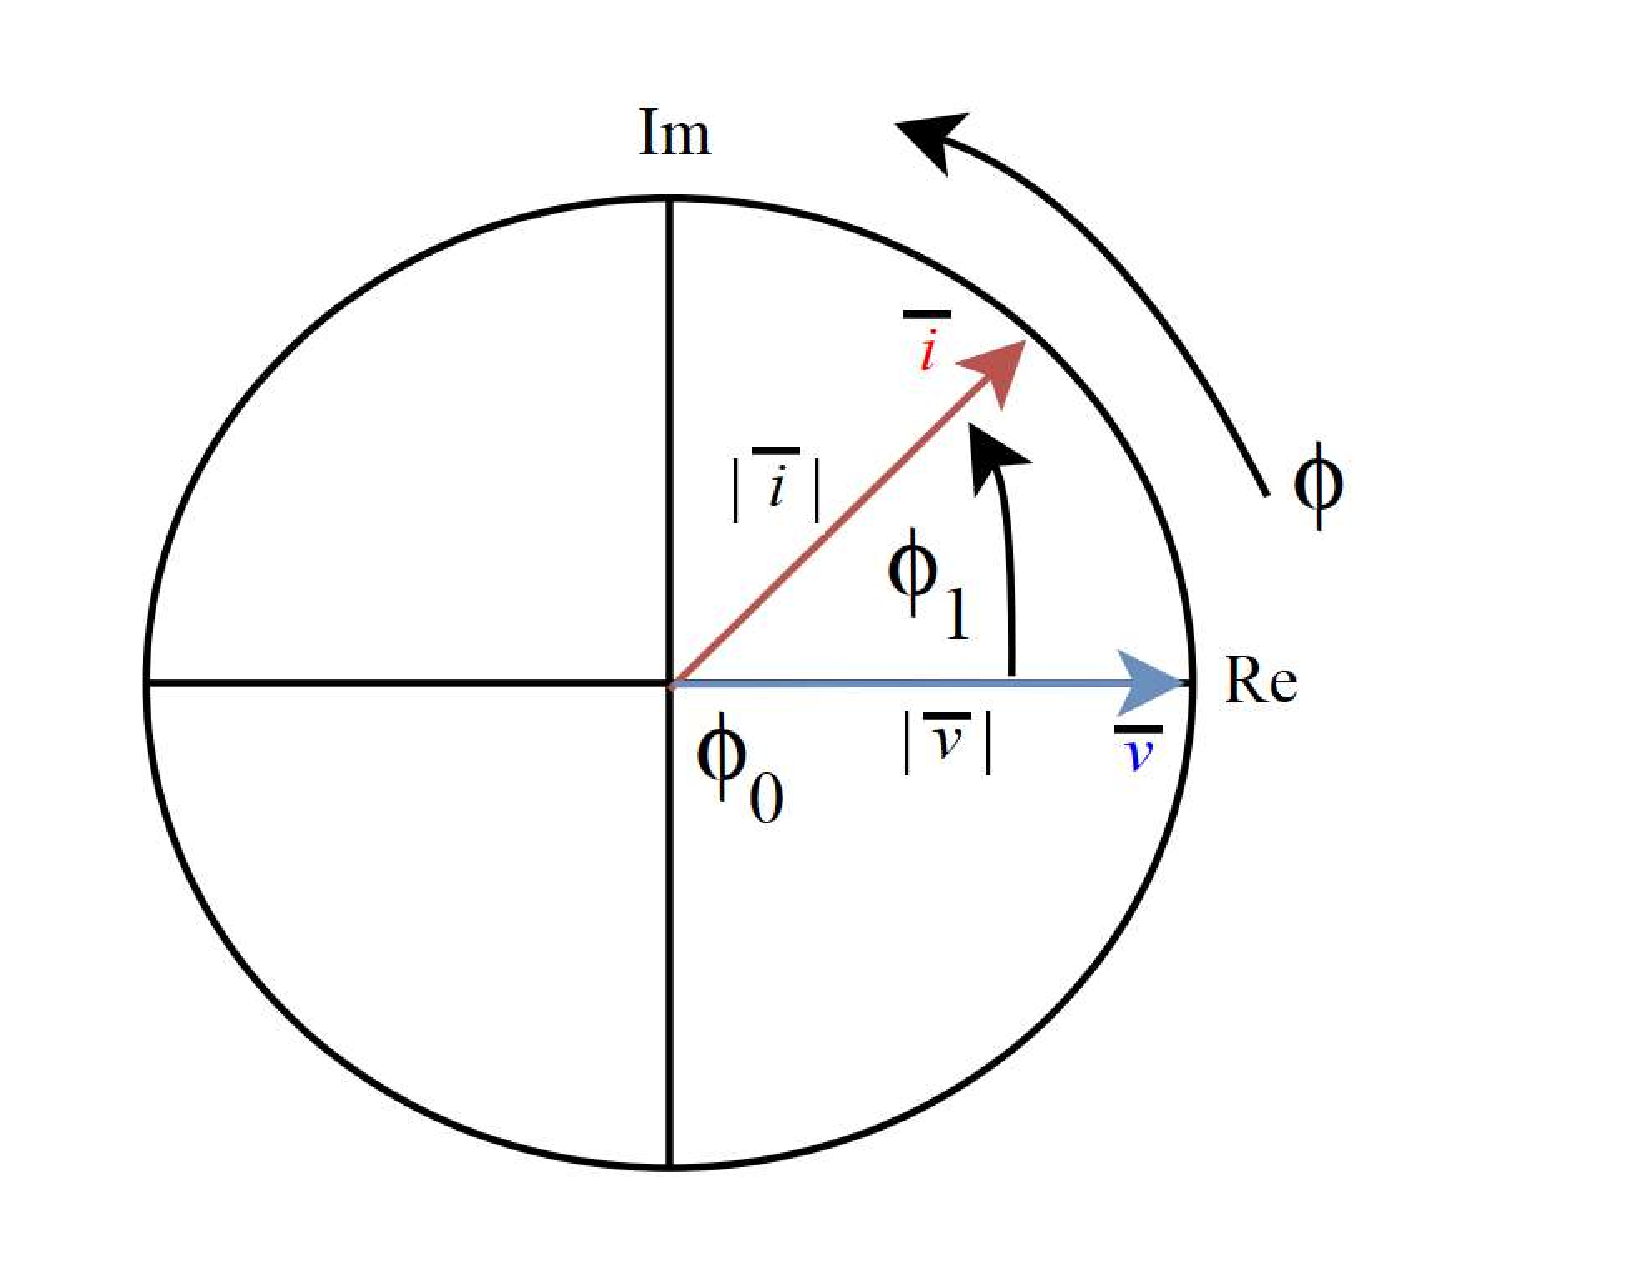
\includegraphics[clip, trim=0 0 0 0, width=0.60\textwidth]{Sections/4_TechnicalAnalysis/Figures/4_1_CapacitancePhasor.pdf}
    \caption{A capacitance causes the current $\bar i$ to lead the voltage $\bar v$. The black $\phi$ arrow signifies the positive direction of the coordinate system.}
    \label{fig:4_1_CapPhasor}
\end{figure}

The voltage vector, $\bar v$, with the phase $\phi_0 = 0$ relative to the real axis, will be the reference for the system because in impedance analyzers the input signal to the DUT will, most often, be a controlled voltage with a known phase and the DUT's phase will be relative to this input waveform. The phase difference $\Delta \phi = \phi_0 - \phi_1$ will correspond to the phase of the $\bar i$ current waveform. The phase of the reference waveform is $\phi_0 = 0$ and this gives the phase of $\bar i$ as shown in eq \ref{eq:4_1_CapPhase}.

\begin{equation}\label{eq:4_1_CapPhase}
    \Delta \phi = \phi_1 - \phi_0=\phi_1 \bigg\rvert_{\phi_0 = 0}
\end{equation}

The impedance of a DUT is the relationship between the voltage and current phasors as shown in equation \ref{eq:4_1_Impedance}.
\begin{equation}\label{eq:4_1_Impedance}
    \bar Z_c = \frac{|\bar v| [cos(\phi_0) +j\cdot sin(\phi_0)]}{|\bar i| [cos(\Delta \phi) +j\cdot sin(\Delta \phi)]}
\end{equation}

Using $\phi_0 = 0$ and $\Delta \phi = \phi_1$ in equation \ref{eq:4_1_Impedance} gets equation \ref{eq:4_1_CapImpedance2}. The numerator reduces to $|\bar v|$ as $cos(0) =1$ and $sin(0) = 0$.
\begin{equation}\label{eq:4_1_CapImpedance2}
    \bar Z_c = \frac{|\bar v|}{|\bar i| [cos(\phi_1) +j\cdot sin(\phi_1)]}
\end{equation}

Applying Eulers formula, and the reciprocal, to eq \ref{eq:4_1_CapImpedance2} gives the final expression for the impedance of a capacitive DUT shown in eq \ref{eq:4_1_CapImpedance4}.
\begin{equation}\label{eq:4_1_CapImpedance4}
    \bar Z_c = \frac{|\bar v|}{|\bar i|} \cdot \mathrm e^{-j\phi_1} = |\bar Z| \cdot \mathrm e^{-j\phi_1} 
\end{equation}
Plotting the impedance vector of a DUT dominated by a capacitance will give a vector pointing into the 4th quadrant as shown in figure \ref{fig:4_1_CapImpedance}.
\begin{figure}[H]
    \centering
    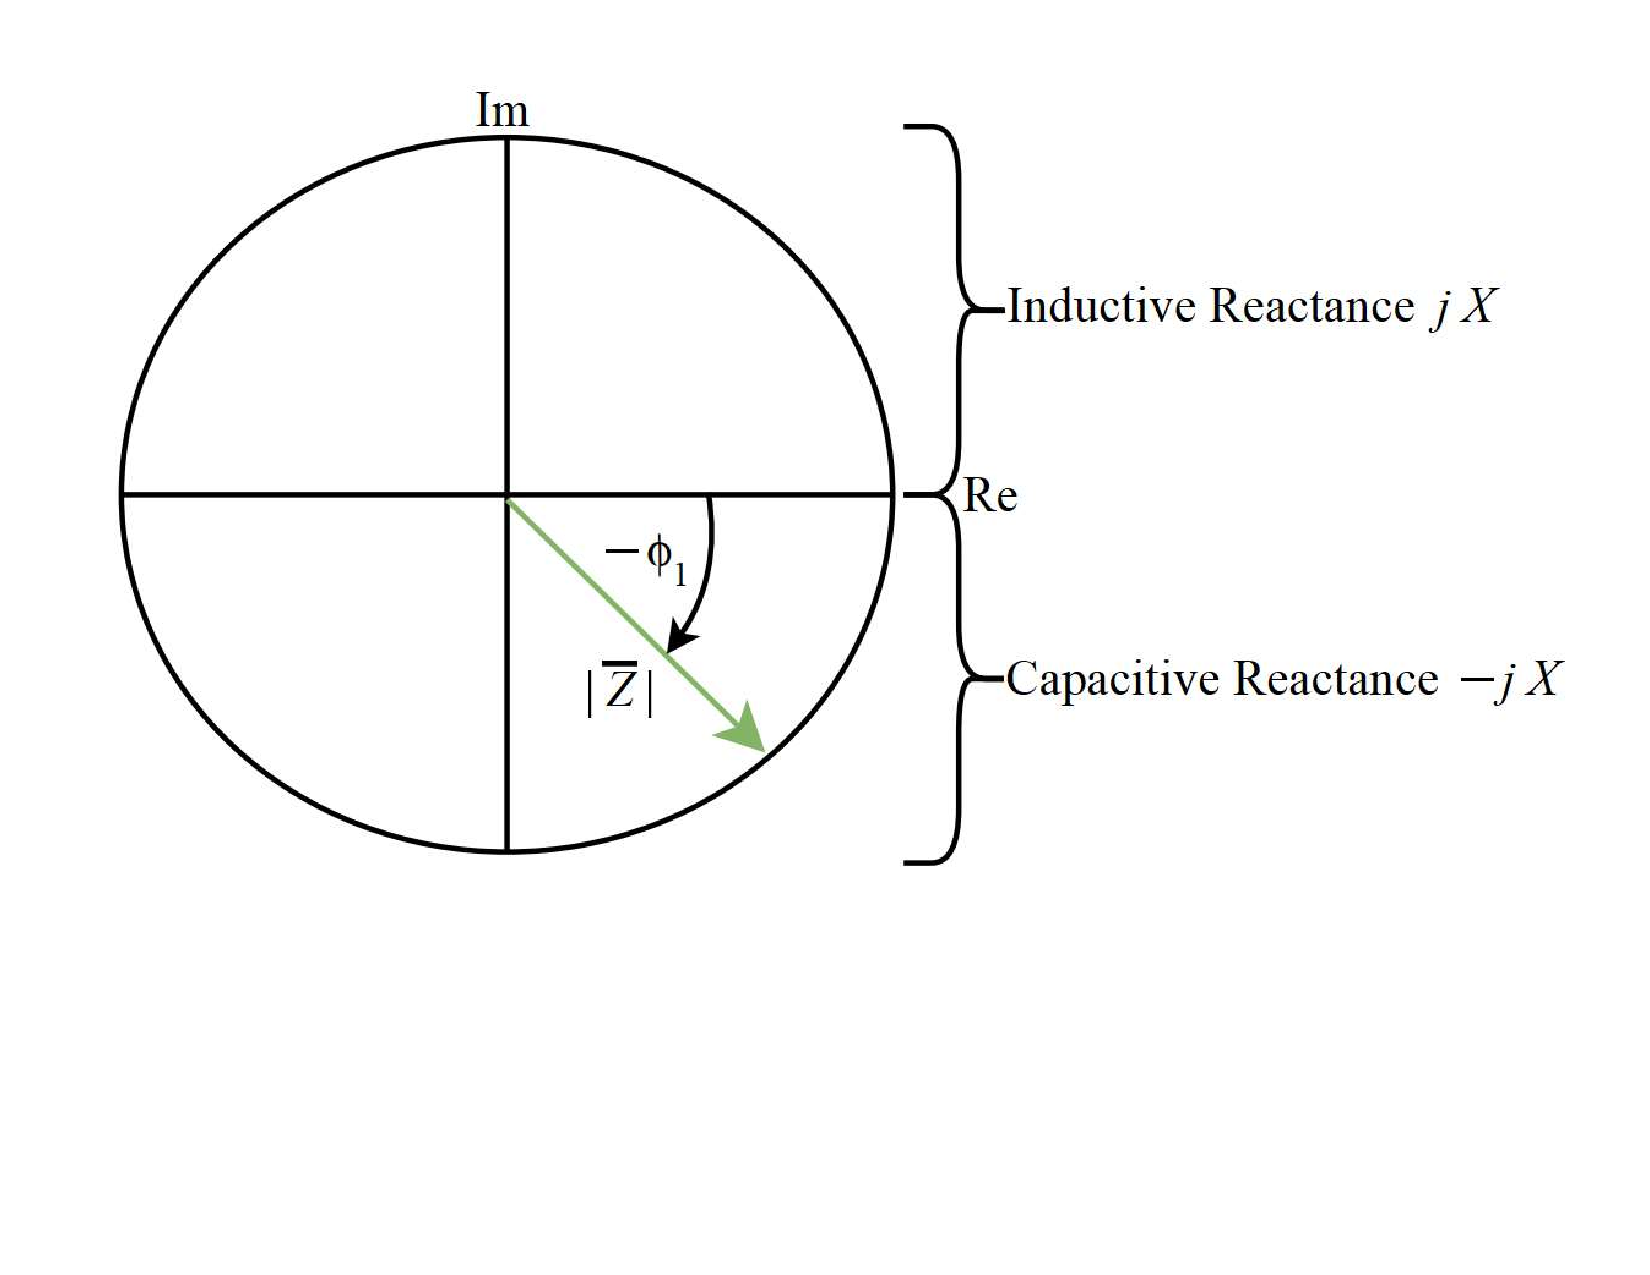
\includegraphics[clip, trim=0 175 0 0, width=0.60\textwidth]{Sections/4_TechnicalAnalysis/Figures/4_1_CapImpedance.pdf}
    \caption{The impedance vector of a capacitive DUT will be located in the 4th quadrant as shown by the $\bar Z$ vector. An impedance pointing into the 4th quadrant is denoted a \textit{capacitive reactance} while an impedance in the 1st quadrant is called a \textit{inductive reactance}.}
    \label{fig:4_1_CapImpedance}
\end{figure}

As shown by figure \ref{fig:4_1_CapImpedance} the sign of the imaginary part of the complex impedance $Z = R \pm jX$ will be an important part to track in order to identify the type of DUT. A similar analysis can be performed with an inductive DUT, in this case the current will lag the voltage as shown on the phasor diagram on figure \ref{fig:4_1_IndPhasor}.
\begin{figure}[H]
    \centering
    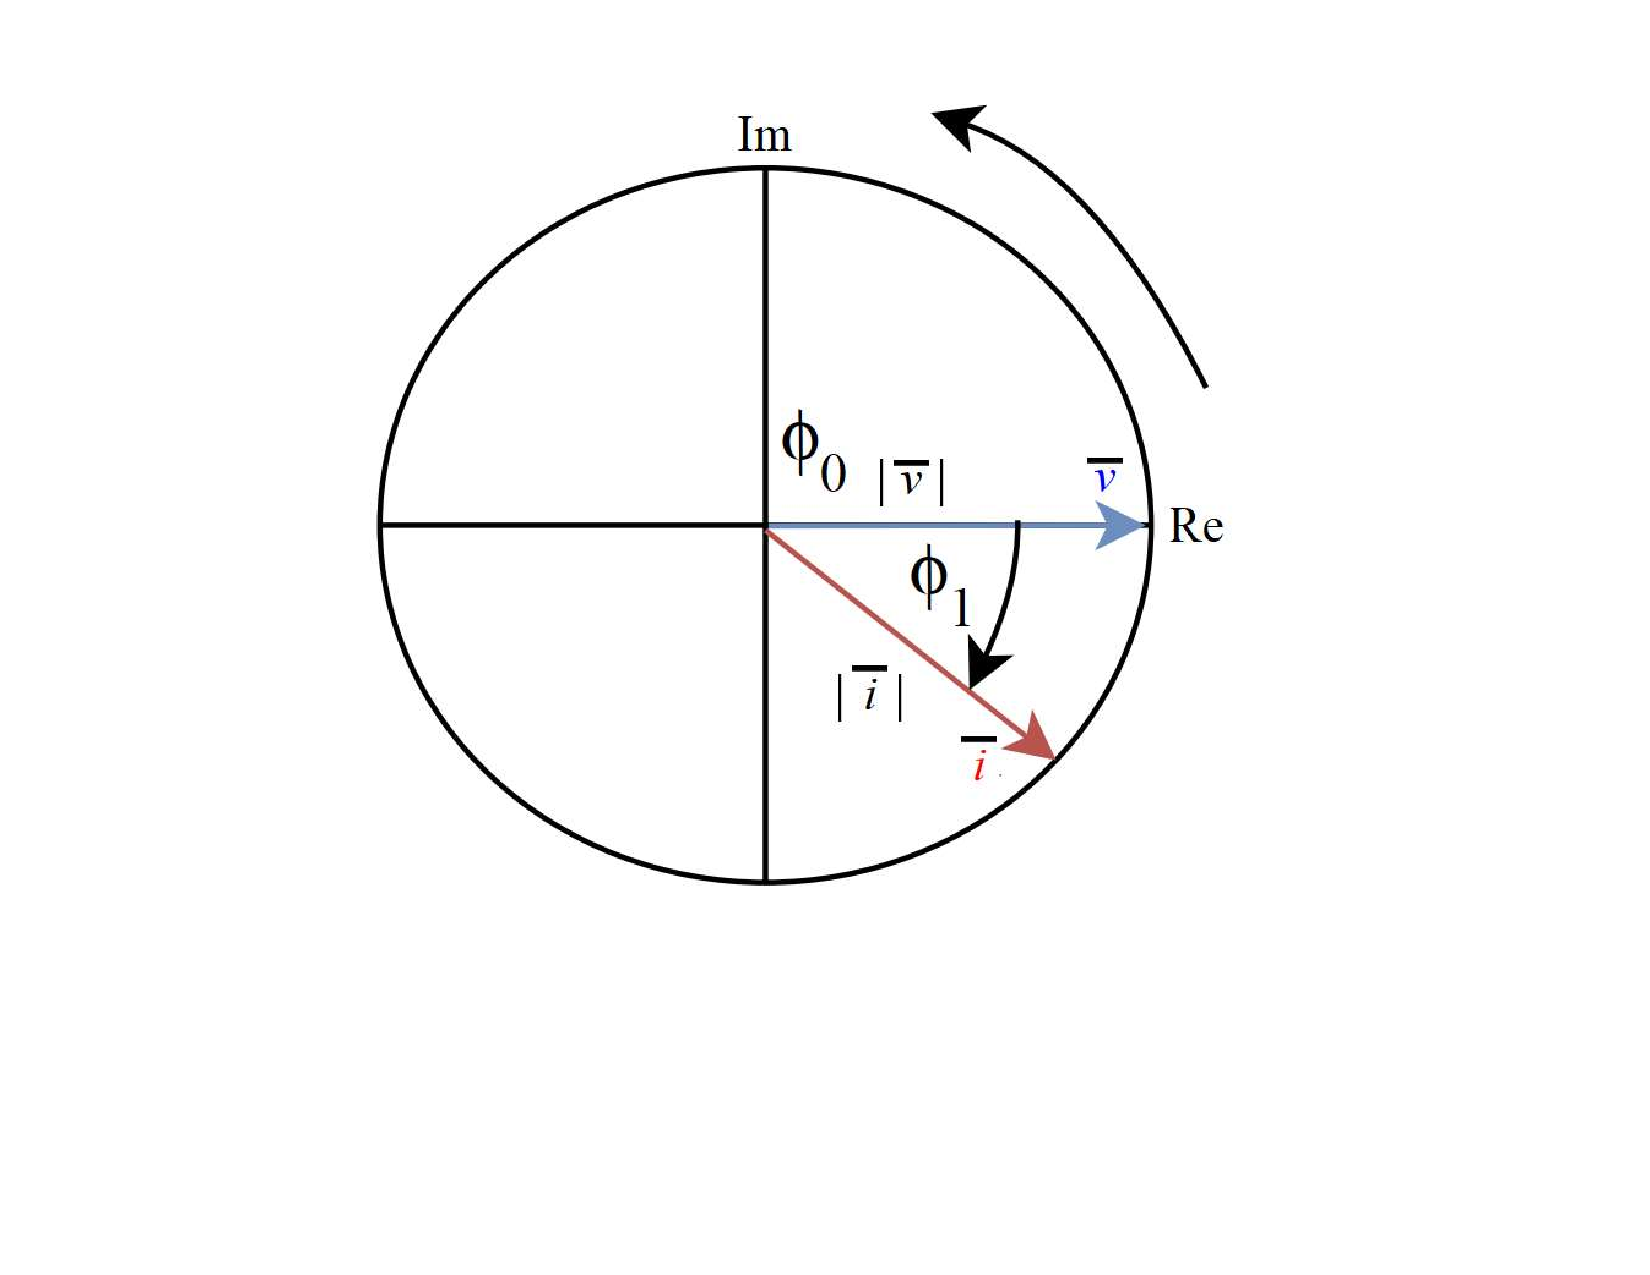
\includegraphics[clip, trim=0 175 0 0, width=0.75\textwidth]{Sections/4_TechnicalAnalysis/Figures/4_1_InductivePhasor.pdf}
    \caption{For an inductive DUT the voltage waveform will lead the current waveform. Note how the phase angle $\phi_1$ of $\bar i$ is going against the established positive direction of the coordinate system.}
    \label{fig:4_1_IndPhasor}
\end{figure}

The current phasor $\bar i$ is lagging the voltage phasor $\bar v$ by a negative phase angle relative to the positive direction of the phasor diagram and will have the phase angle shown in eq \ref{eq:4_1_IndPhase}.

\begin{equation}\label{eq:4_1_IndPhase}
    \Delta \phi = \phi_0 -(-\phi_1) =\phi_1 \bigg\rvert_{\phi_0 = 0}
\end{equation}

Applying eq \ref{eq:4_1_IndPhase} to eq \ref{eq:4_1_Impedance} gives the impedance of an inductive DUT as shown in 
\begin{equation}\label{eq:4_1_IndImpedance2}
    \bar Z_l = \frac{|\bar v|}{|\bar i| [cos(\phi_1) -j\cdot sin(\phi_1)]}
\end{equation}
Once again apply Eulers formula like in eq \ref{eq:4_1_CapImpedance4} on eq \ref{eq:4_1_IndImpedance2} gives eq \ref{eq:4_1_IndImpedance3}

\begin{equation}\label{eq:4_1_IndImpedance3} 
    \bar Z_l = \frac{|\bar v|}{|\bar i|} \cdot \frac{1}{cos(\phi_1) - j\cdot sin(\phi_1)} = |\bar Z| \cdot \mathrm (e^{-j\phi})^{-1}
\end{equation}
Eq \ref{eq:4_1_IndImpedance3} is simplified to equation \ref{eq:4_1_IndImpedance4}.
\begin{equation}\label{eq:4_1_IndImpedance4} 
    \bar Z_l =|\bar Z| \cdot \mathrm e^{j\phi}
\end{equation}
Equation \ref{eq:4_1_IndImpedance4} has positive phase and is an impedance vector now pointing into the first quadrant which signifies that it has inductive reactance as shown on figure \ref{fig:4_1_IndImpedance}.

\begin{figure}[H]
    \centering
    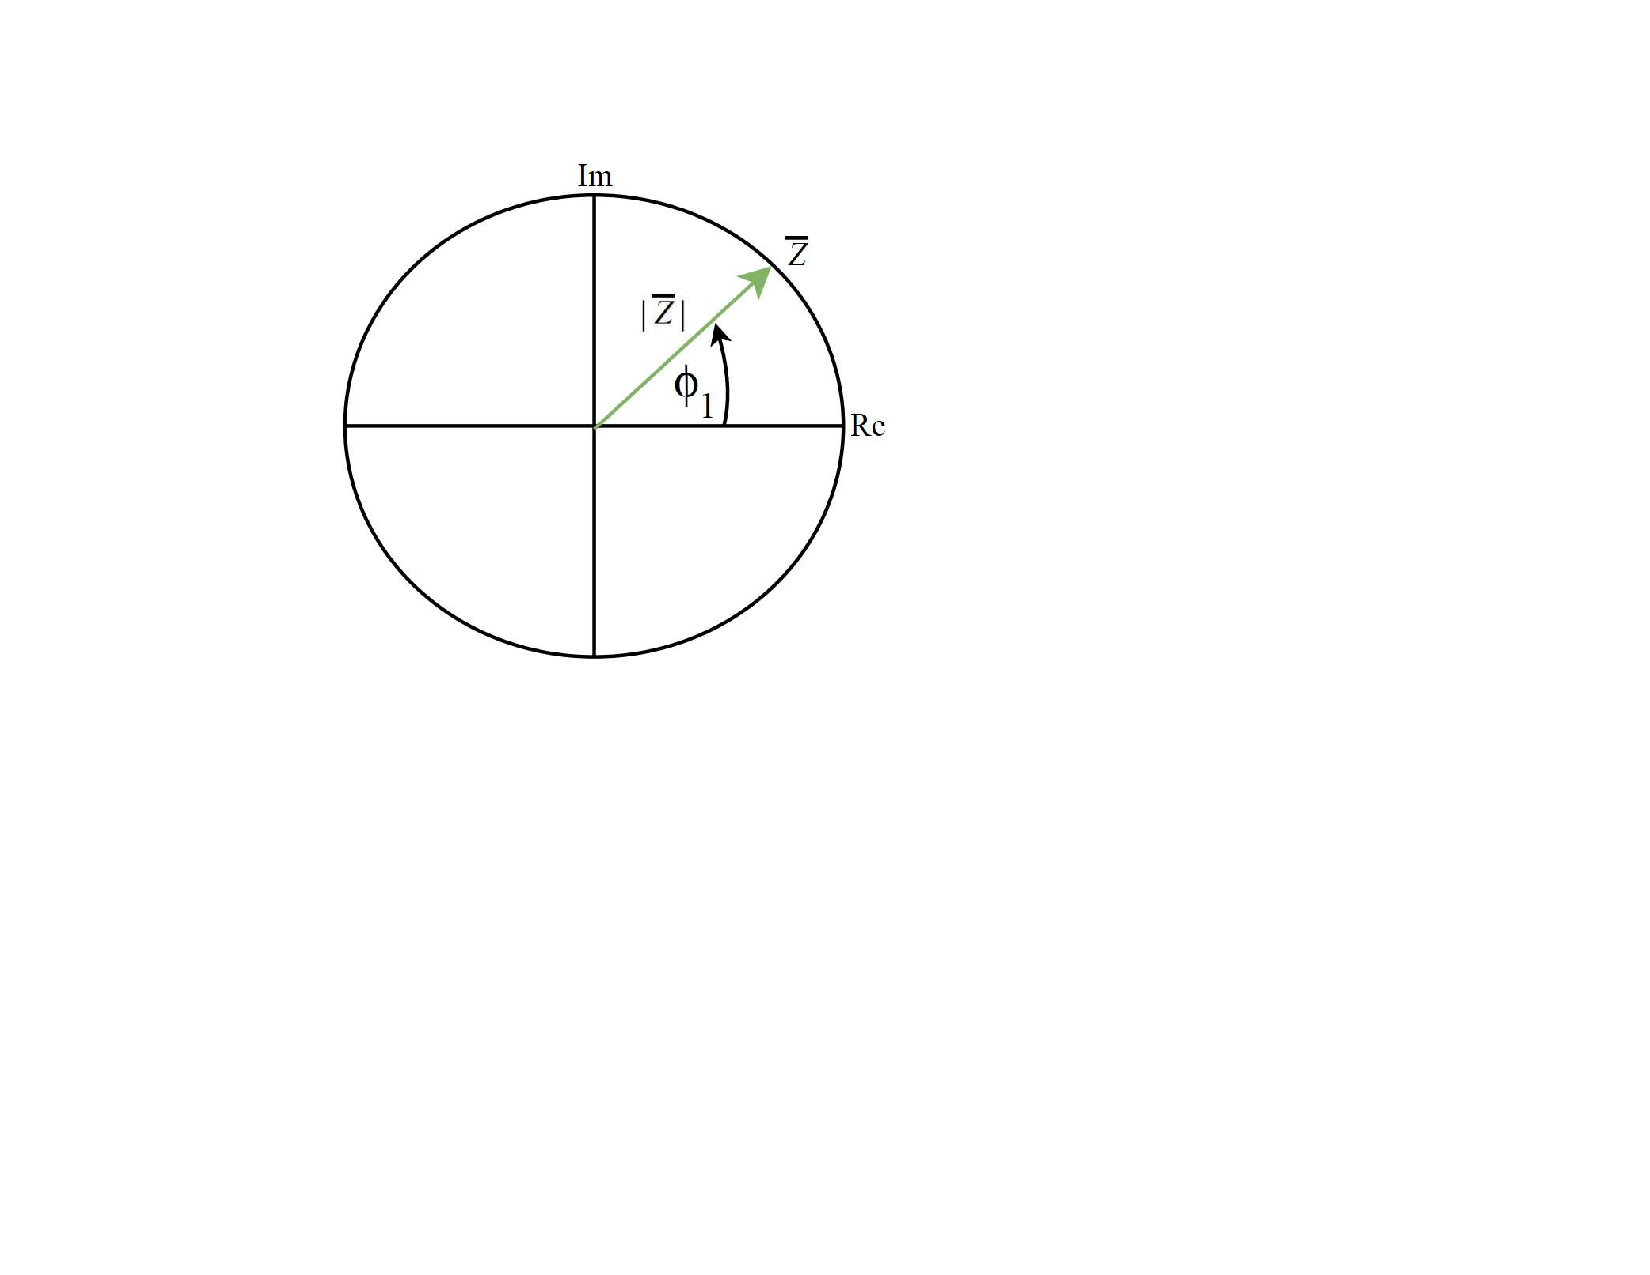
\includegraphics[clip, trim=0 275 0 0, width=1\textwidth]{Sections/4_TechnicalAnalysis/Figures/4_1_IndImpedance.pdf}
    \caption{The impedance an of inductive DUT is pointing into the first quadrant which means the impedance has inductive reactance.}
    \label{fig:4_1_IndImpedance}
\end{figure}
